\documentclass[11pt,letterpaper]{article}
\usepackage[latin1]{inputenc}
\usepackage{amsmath}
\usepackage{amsfonts}
\usepackage{amssymb}
\usepackage{graphicx}
\usepackage{capt-of}

\setlength{\parskip}{1pc}
\setlength{\parindent}{0pt}
\setlength{\topmargin}{-3pc}
\setlength{\textheight}{9.0in}
\setlength{\oddsidemargin}{0pc}
\setlength{\evensidemargin}{0pc}
\setlength{\textwidth}{6.5in}

\title{6.170 Assignment 2: Object Models}
\author{Dina Betser}


\begin{document}
\maketitle

\section{Background}
\begin{enumerate}
\item Entity Relationship Model\\
ER modeling is used to describe the type of information that is to be stored in a database. Objects are represented as ``entities''.
\item Object Modeling Technique\\
This was developed as a method to develop object-oriented systems and to support OOP. Objects and their relationships are expressed using multiplicities.
\item Software Analysis Patterns\\
This modeling technique aims to represent ideas that have been useful in one practical context and will probably be useful in others.
\item Unified Modeling Language\\
The most sophisticated of the languages listed, UML is a standard modeling language that has a lot of the same characteristics as the object modeling notation used in this class, including inheritance.
\end{enumerate}

One feature that is present in all modeling formats except for ER modeling is inheritance/generalization.

\section{Conceptual modeling problems}
\begin{itemize}
\item Prerequisites. Model the relationships between classes and their prerequisites. Note that there may be different ways in which the prerequisites of a class can be satisfied; for example, two prerequisite classes may be interchangeable.\\

\begin{enumerate}
\item Ambiguities Resolved\\
The fact that multiple combinations of prerequisites can satisfy the prerequisites of a given class was disambiguated by 

\item Complexities Ignored\\
Assumed that

\item Designations\\
A \texttt{Credit} is defined as some form of knowledge that satisfies a given prerequisite. This could be in the form of transfer credit from another school, a


\item Object Model\\
\begin{center}
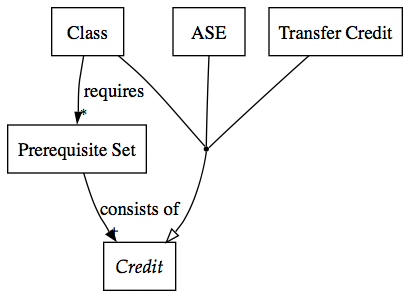
\includegraphics[width=200pt]{dot/b1.png}
\label{fig:ob1} 
\end{center}
\end{enumerate}

\item Street map. Model a street map that includes named streets and their intersections, and the notion of one-way streets and divided highways. Note in particular that one street may be accessible from an intersecting street only for traffic moving in a particular direction.

\begin{enumerate}
\item Ambiguities Resolved\\

\item Complexities Ignored\\

\item Designations\\

\item Object Model\\
\begin{center}
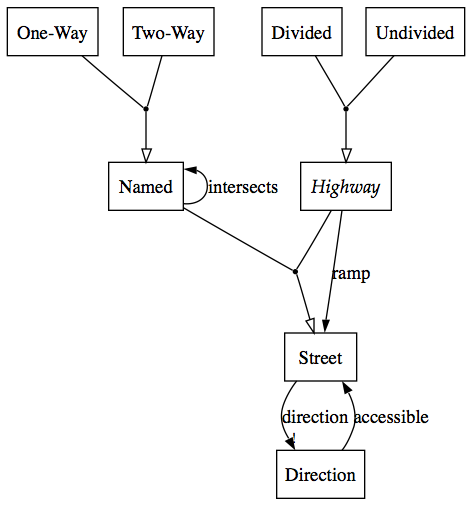
\includegraphics[width=300pt]{dot/b2.png}
\label{fig:ob2} 
\end{center}
\end{enumerate}

\item Voting ballots. Model the ballots cast in a voting scheme, in which on each ballot the voter makes choices of candidates for a variety of offices.

\begin{enumerate}
\item Ambiguities Resolved\\

\item Complexities Ignored\\

\item Designations\\

\item Object Model\\
\begin{center}
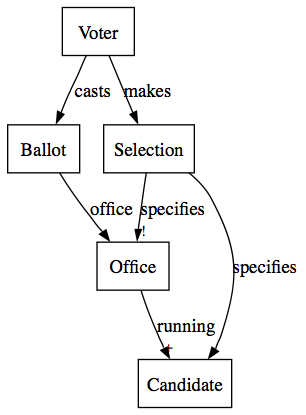
\includegraphics[width=200pt]{dot/b3.png}
\label{fig:ob3} 
\end{center}
\end{enumerate}

\item Java types. Model the type structure of objects in a Java program, in which there are two kinds of types, class types and interfaces, related by implements and extends. Include in your model a notion of variables, each with a declared type and containing an object of a given type. What is the relationship between the two types?\\

\begin{enumerate}
\item Ambiguities Resolved\\

\item Complexities Ignored\\

\item Designations\\

\item Object Model\\
\begin{center}
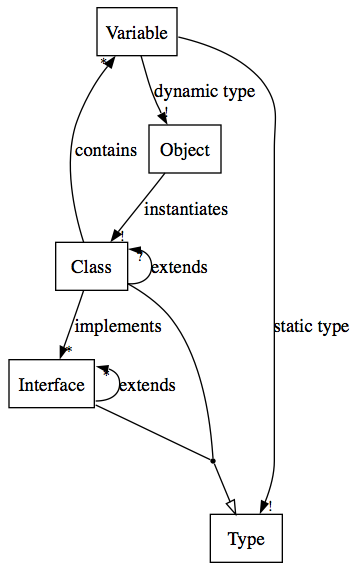
\includegraphics[width=200pt]{dot/b4.png}
\label{fig:ob4} 
\end{center}
\end{enumerate}

\end{itemize}



\section{Modeling Python Modules}
\begin{enumerate}
\item Ambiguities Resolved\\

\item Complexities Ignored\\

\item Designations\\

\item Object Model\\
\begin{center}
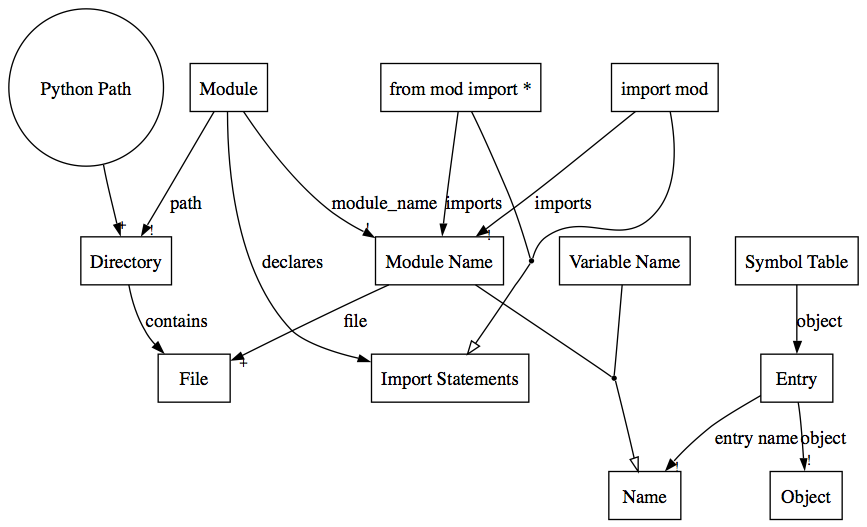
\includegraphics[width=500pt]{dot/pythonmodules.png}
\label{fig:ob5}
\end{center}
\end{enumerate}

\section{Extracting an OM from an API}
\begin{enumerate}
\item Ambiguities Resolved\\

\item Complexities Ignored\\

\item Designations\\

\item Object Model\\
\begin{center}
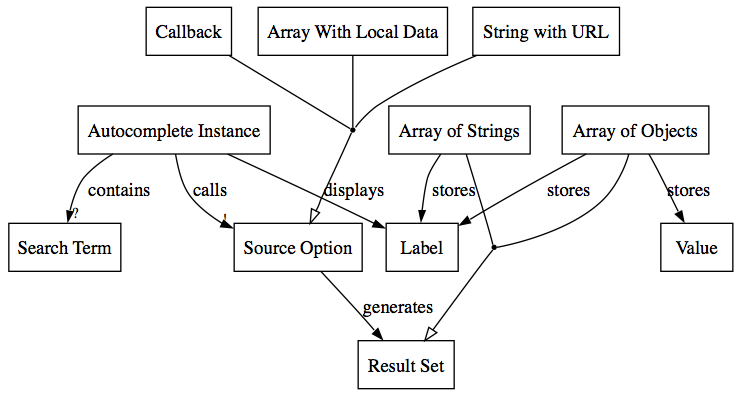
\includegraphics[width=400pt]{dot/autocomplete.png}
\label{fig:ob6} 
\end{center}
\end{enumerate}

\section{Metamodeling}
\begin{enumerate}
\item Ambiguities Resolved\\
It was ambiguous whether the ``disjoint set'' relationship referred to the parent-child subset relationship, or among children in a parent-child subset relationship. I chose to assume the latter, so Sets are described as disjoint with respect to other sets.

\item Complexities Ignored\\
In the modified version of the metamodeling object model, I've created a ``disjoint set''
\item Designations\\

\item Object Models\\
Part 1:
\begin{center}
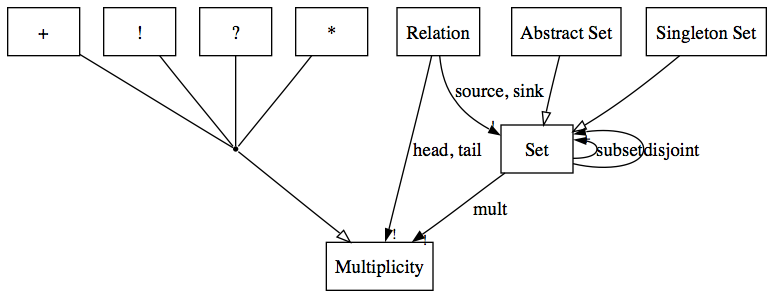
\includegraphics[width=400pt]{dot/metamodeling.png}
\label{fig:ob7} 
\end{center}

Part 2:
\begin{center}
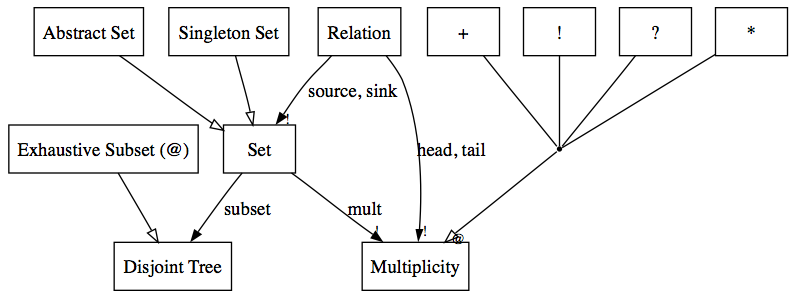
\includegraphics[width=400pt]{dot/metamodeling2.png}
\label{fig:ob8} 
\end{center}
\end{enumerate}

\end{document}

